\documentclass[12pt,]{article}
\usepackage{lmodern}
\usepackage{amssymb,amsmath}
\usepackage{ifxetex,ifluatex}
\usepackage{fixltx2e} % provides \textsubscript
\ifnum 0\ifxetex 1\fi\ifluatex 1\fi=0 % if pdftex
  \usepackage[T1]{fontenc}
  \usepackage[utf8]{inputenc}
\else % if luatex or xelatex
  \ifxetex
    \usepackage{mathspec}
    \usepackage{xltxtra,xunicode}
  \else
    \usepackage{fontspec}
  \fi
  \defaultfontfeatures{Mapping=tex-text,Scale=MatchLowercase}
  \newcommand{\euro}{€}
    \setmainfont{Georgia}
\fi
% use upquote if available, for straight quotes in verbatim environments
\IfFileExists{upquote.sty}{\usepackage{upquote}}{}
% use microtype if available
\IfFileExists{microtype.sty}{%
\usepackage{microtype}
\UseMicrotypeSet[protrusion]{basicmath} % disable protrusion for tt fonts
}{}
\usepackage[hmargin=1in,vmargin=1in]{geometry}
\usepackage{graphicx}
\makeatletter
\def\maxwidth{\ifdim\Gin@nat@width>\linewidth\linewidth\else\Gin@nat@width\fi}
\def\maxheight{\ifdim\Gin@nat@height>\textheight\textheight\else\Gin@nat@height\fi}
\makeatother
% Scale images if necessary, so that they will not overflow the page
% margins by default, and it is still possible to overwrite the defaults
% using explicit options in \includegraphics[width, height, ...]{}
\setkeys{Gin}{width=\maxwidth,height=\maxheight,keepaspectratio}
\ifxetex
  \usepackage[setpagesize=false, % page size defined by xetex
              unicode=false, % unicode breaks when used with xetex
              xetex]{hyperref}
\else
  \usepackage[unicode=true]{hyperref}
\fi
\hypersetup{breaklinks=true,
            bookmarks=true,
            pdfauthor={Instructor: Michael Treglia},
            pdftitle={Finding, Downloading, and Working With GIS Data in QGIS for (mostly) the United States},
            colorlinks=true,
            citecolor=blue,
            urlcolor=blue,
            linkcolor=magenta,
            pdfborder={0 0 0}}
\urlstyle{same}  % don't use monospace font for urls
\setlength{\parindent}{0pt}
\setlength{\parskip}{6pt plus 2pt minus 1pt}
\setlength{\emergencystretch}{3em}  % prevent overfull lines
\setcounter{secnumdepth}{0}

\title{Finding, Downloading, and Working With GIS Data in QGIS for (mostly) the
United States}
\author{Instructor: Michael Treglia}
\date{Landscape Analysis and Modeling, The University of Tulsa, Spring 2015}

\begin{document}
\maketitle

*Note: This material is available online with active hyperlinks at
\url{http://mltconsecol.github.io/TU_LandscapeAnalysis_Documents/Assignments_web/Assignment02_AccessingGISData.html}

\section{Accessing Ecologically-relevant GIS
Datasets}\label{accessing-ecologically-relevant-gis-datasets}

Though many studies use various spatial/GIS datasets, finding and
working with them can be a bit of a mystery to a GIS newcomer. This
document is designed to point users in the right direction to get
started, with a focus on the United States (though some datasets
discussed here are also available for other parts of the world). The
resources listed below are not necessarily mutually-exclusive to
one-another (i.e, you can often find some of the same datasets at
multiple places), though some datasets may only be available from
individual sources. Detailed instructions on downloading the data are
given for the first source to familiarize users with data downloads, but
they should explore the other websites to try and figure out how to
access the data there - unfortunately every website is a bit different.
Typically the projection information is provided and will be read by
your GIS software, but if it is not, you may need to look into metadata
that comes with the files. This document is meant to get users started,
and is thus not to serve as a comprehensive manual for accessing every
data source available. Remember - Google is your friend. If it helps,
start at these websites to look for datasets you need; if you can't find
them, they may exist, but that might require some web-searches. Also,
internet Q\&A outlets like \href{http://gis.stackexchange.com/}{GIS
Stack Exchange} are invaluable when you really get stuck.

\subsection{National-Scale Data}\label{national-scale-data}

\subsubsection{The National Map}\label{the-national-map}

\href{http://nationalmap.gov/}{The National Map} is kind of a
one-stop-shopping location for lots of datasets that are distributed by
the U.S. Government. These include vector layers of political
boundaries, hydrologic data including stream networks and watershed
boundaries from the \href{http://nhd.usgs.gov/}{National Hydrography
Dataset}, and roads. These layers are typically available for download
as shapefiles or geodatabase files. Raster datasets that are available
include elevation (digital elevation models {[}DEMs{]}) from the
\href{http://ned.usgs.gov/}{National Elevation Dataset}, land cover
classifications from the \href{http://www.mrlc.gov/}{National Land Cover
Database}, and aerial imagery.

The National Map has lots of ways to view and download data, with
semi-regular improvements. You should take some time and explore
\href{http://nationalmap.gov/}{The National Map website} for yourself,
but a good way to see what is available is through the Data Download and
Visualization Services - The National Map Download Platform -
\url{http://viewer.nationalmap.gov/basic/} (pictured below).

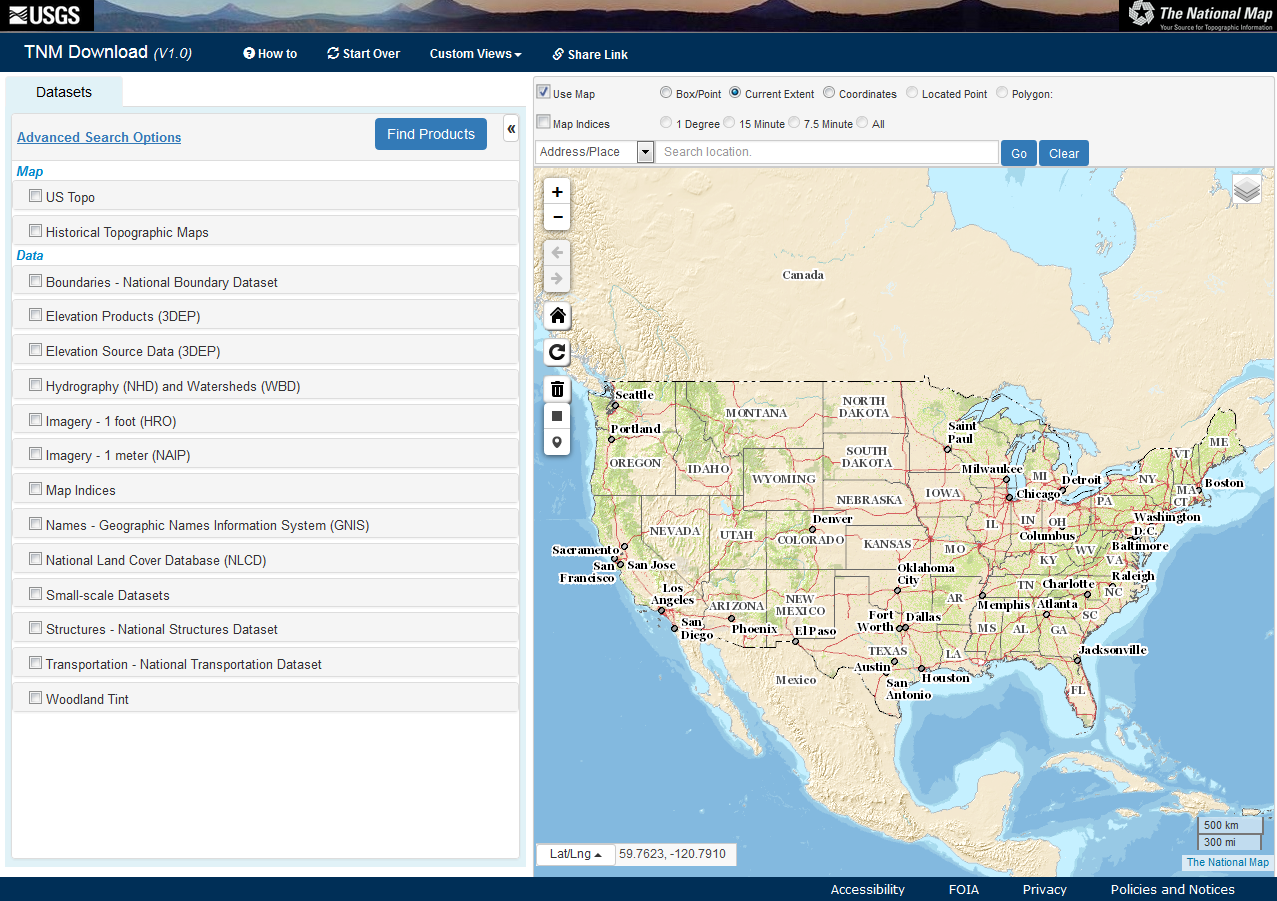
\includegraphics{../Assignment_Images/TNM_DownloadPlatform.PNG}\\ On the
left hand panel, you will see a list of existing maps and data that
might be avaialble for your areas of interest. The \emph{Map} categories
are provided as PDFs or GeoPDFs, ready to use in the field. The
\emph{Data} categories are GIS files, that can be brought into QGIS (or
other GIS software) for manipulation, analysis, and visualization.

. Browse this page - hover your mouse over the icons just above the the
map to see what they do, and expand the lists of layers on the left by
clicking the + and - icons next to the categories. Check and un-check
the boxes to see what these data look like; use the scroll-wheel on your
mouse, or the magnifying glass with the + in it to adjust the zoom. You
can also search for specific places in the search bar at the top. Note,
for the layers labeled ``\ldots{} Availability'', this will show
polygons representing areas that the data are available for, as the
layers themselves can be complex. However, when you go to download data,
you will be able to download the actual layers.

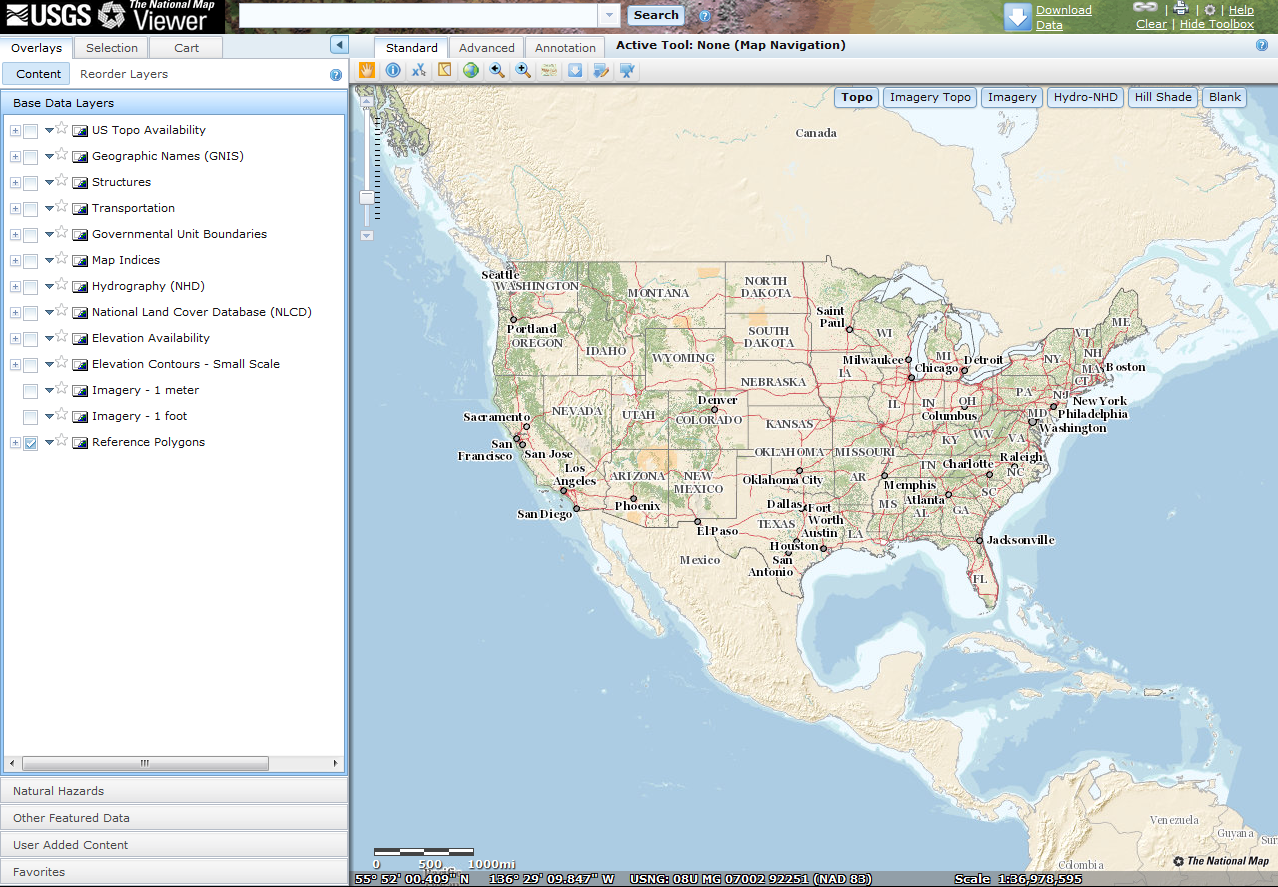
\includegraphics{../Assignment_Images/TNM_Image.PNG}\\

\paragraph{Downloading Data from The National
Map}\label{downloading-data-from-the-national-map}


\includegraphics{./Images/TNM_DownloadIcon.png}~To begin the process of
downloading data from The National Map, simply click one of the
``Download Data'' icons, either at the top of the webpage, or just above
the map window (in a row with other icons). You do not need to have the
layers you want to download visible on your map; you will select the
layers in a later step.

You can select any of the appropriate options for defining the extent of
data you wish to download. For beginners to GIS, the simplest ways are
likely:

\begin{itemize}
\itemsep1pt\parskip0pt\parsep0pt
\item
  draw and download by bounding box;
\item
  download by current map extent; or
\item
  download by coordinate input.
\end{itemize}

In this example, we'll focus on a natural area near our campus, Turkey
Mountain. A search for ``Turkey Mountain, Tulsa, OK'' yields a fairly
accurate result. Zoom to the appropriate area, and select the option to
download data by drawing a bounding box (the first option). Here's an
image of the bounding box I have selected:

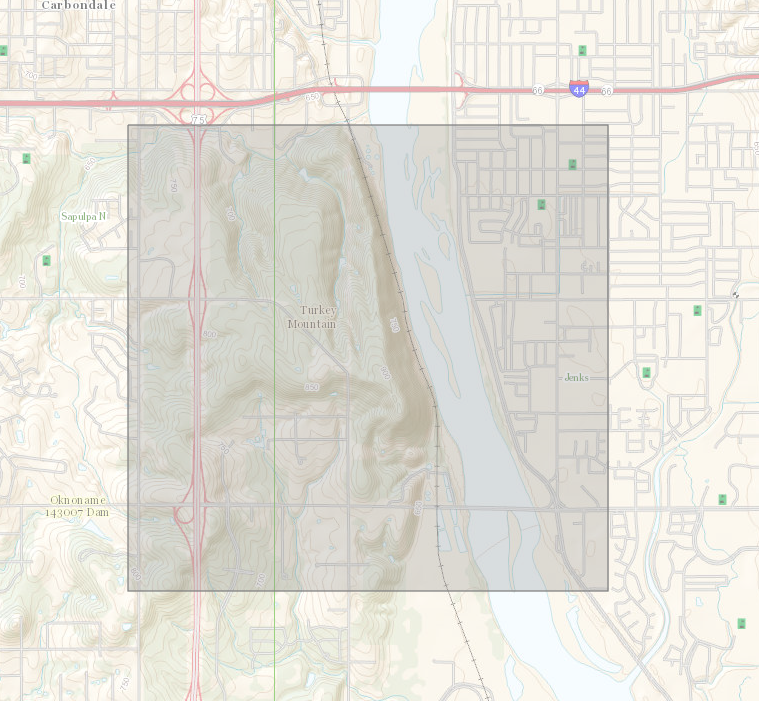
\includegraphics{./Images/TNM_BoundingBoxDownload.PNG}\\ After you draw
the box, a new window will appear with check-boxes of data you want to
download. For now, lets check the options for ``Boundaries'' and
``Elevation'' and click ``Next'' (read the on-page instructions at this
point if you are having issues).

A new window should now appear (image below), with lots of products
available to download (right now you are only looking at the
``Boundaries'' products; you'll need to click the gray ``Elevation''
category to access those). Admittedly, this can be a bit overwhelming,
and it might take a bit of trial and error to figure out what you need.
In most contexts, for vector data, shapefiles are the easiest to work
with, but you might need to download a ``File GDB'' option instead. In
this case, the third option, ``USGS National Boundary Dataset (NBD) for
Oklahoma 20140401 State or Territory Shapefile'' might suffice, but if
you want the fine-scale map of cities and towns, scroll down to that
option as well. Check the box for both of those. If data are available
for multiple dates, but they otherwise look the same, get the most
recent, or most appropriate for your focal time period.

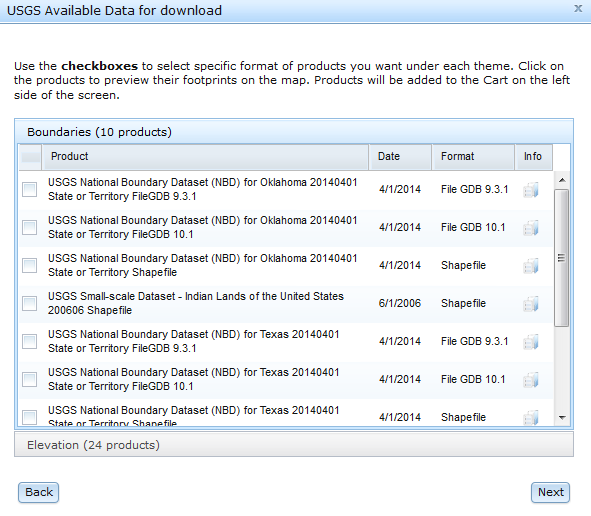
\includegraphics{./Images/TNM_LayerSelection.PNG}\\ Next, open the tab
for ``Elevation'' - again, there are lots of options. Notice that in the
product name, it typically says ``1 arc-second'', ``1/3 arc-second'' or
``100 {[}or 200{]}-Meter Resolution'' - this identifies the resolution
(i.e., grain size), as these are raster layers. 1 arc-second is
\textasciitilde{}30 meters x 30 meters and 1/3 arc-second is
\textasciitilde{}10 meters x 10 meters. You'll notice there are also a
number of formats available. GeoTIFF or IMG files are typically among
the easiest to open, with the projection information embedded and
nothing to do but import those in QGIS. If you are working with a large
area, you'll have to take notice of the location these are from - in the
name, the n37w096 indicates the latitude/longitude of the upper left
corner of the individual tile. For large areas, it will have multiple
tiles with different latitude/longitude designations, and you'll need to
download all that cover your study area. In this case, we'll select the
``USGS NED n37w096 1 arc-second 2013 1 x 1 degree IMG''.

After you select all desired layers, click the ``Next'' button. (In your
own work, select whatever layers you might need.)

On the left hand side of the screen, ad new panel should be displayed,
the ``Cart'' - you can click on the products you previously selected,
and a preview will appear; you can also remove layers, or opt to add
more. If you are satisfied with the selection, click ``Checkout'' to
move on with your data order. You'll need to enter your e-mail address
twice, and click the ``Place Order'' button. You'll receive download
links in your e-mail, though it can take a little while. The links
typically don't work in Mozilla Firefox, but work to start downloads in
Internet Explorer or Google Chrome.

Once you have the data downloaded, you can import them into your
favorite GIS software.

\subsubsection{USDA GIS Resources}\label{usda-gis-resources}

The \href{http://datagateway.nrcs.usda.gov/}{USDA Geospatial Gateway}
also has a wide variety of data available for download, including soil
data, and high resolution aerial imagery. To get started, go to the
\href{http://datagateway.nrcs.usda.gov/}{website} and click the green
``Get Data'' button (towards the upper-right).

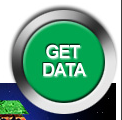
\includegraphics{./Images/USDA_GetData.PNG}~

From there, you'll need to select the desired State/County of interest,
and the datasets you need. see the panes on the left of the screen that
describe each step, as in the example below). Note, this website has
available Climate data from PRISM, further described below.

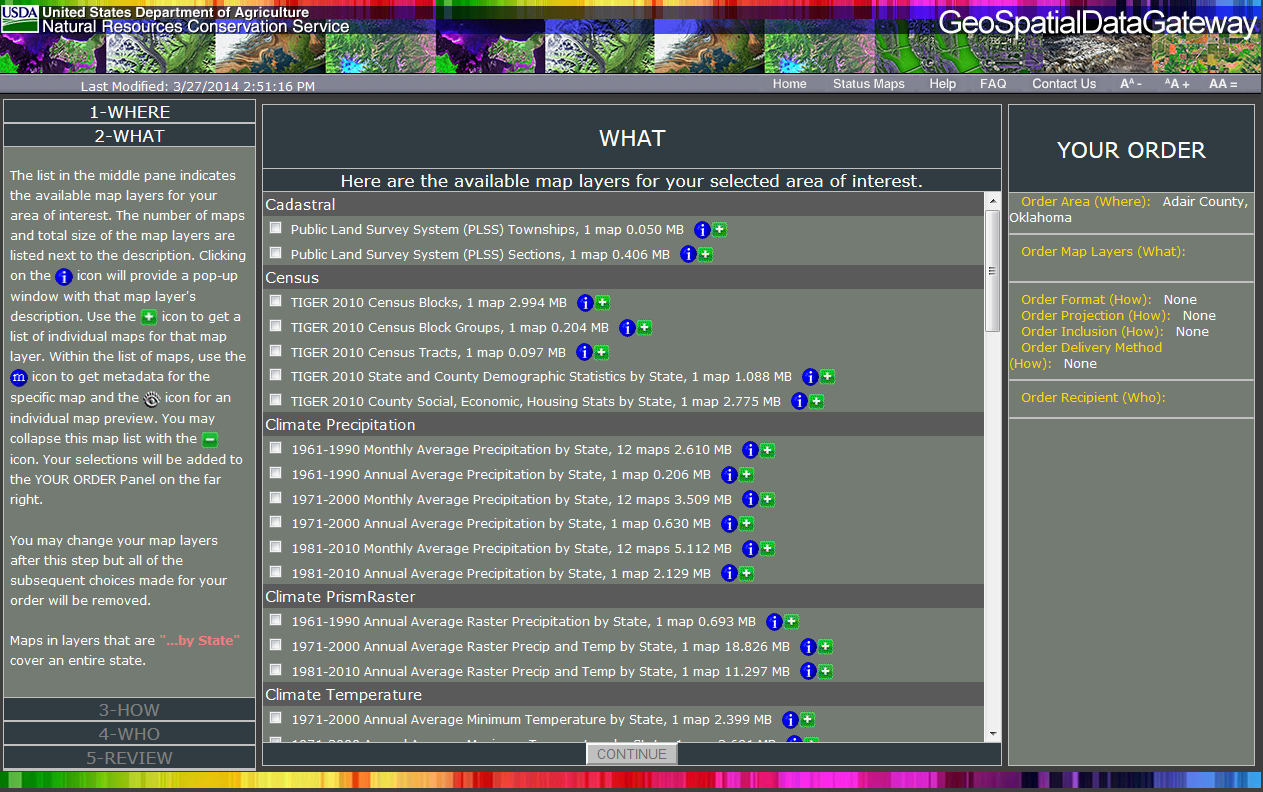
\includegraphics{./Images/USDA_OrderForm.PNG}\\

\subsection{State GIS Resources (for
Oklahoma)}\label{state-gis-resources-for-oklahoma}

Most states have their own repositories for GIS data. Typically when I'm
trying to find such a repository, I do a Google search for something
along the lines of these phrases: ``{[}Insert State Name{]} GIS Data'';
``{[}Insert State Name{]} GIS Repository''; ``{[}Insert State Name{]}
GIS Warehouse''; or ``{[}Insert State Name{]} GIS Clearinghouse''. Here
are also a couple of websites that list some resources available by
state:

\begin{itemize}
\itemsep1pt\parskip0pt\parsep0pt
\item
  \href{http://guides.tulsalibrary.org/content.php?pid=557423\&sid=4599537}{Tulsa
  City-County Library GIS resources}
\item
  \href{http://serc.carleton.edu/NAGTWorkshops/gis/state_resources.html}{Carleton
  College webpage from theNational Association of Geoscience Teachers}
\end{itemize}

For Oklahoma, a couple of particular websites that can be useful are:

\begin{itemize}
\itemsep1pt\parskip0pt\parsep0pt
\item
  \href{http://ogi.state.ok.us/ogi/search.aspx}{The OKMaps Website}
\item
  \href{http://geo.ou.edu/DataFrame.htm}{Center for Spatial Analysis at
  the University of Oklahoma}
\end{itemize}

\subsection{Climate Data}\label{climate-data}

Climate data are typically recorded at individual weather stations,
though in ecological studies, it is typically useful to have summaries
of climate conditions for entire landscapes, describing characteristics
of temperature and precipitation regimes. Thus, multiple organizations
have interpolated the data from weather stations, to estimate conditions
for large areas. There are two main sources I frequently go to, listed
below. Browse the respective website for information on downloading the
data. If you need information from a specific weather station, you can
search the resources from the
\href{http://www.ncdc.noaa.gov/data-access/land-based-station-data}{NOAA
National Climatic Data Center}. Other sources may be available from
state-wide monitoring networks (e.g.,
\href{https://www.mesonet.org/}{Mesonet for Oklahoma} and other
organizations.

\begin{itemize}
\itemsep1pt\parskip0pt\parsep0pt
\item
  \href{http://www.prism.oregonstate.edu/}{PRISM Climate Group at Oregon
  State}

  \begin{itemize}
  \itemsep1pt\parskip0pt\parsep0pt
  \item
    Has 800 meter pixel data for the continental United States
  \item
    Lots of information, including 30 year normals for monthly and
    annual precipitation, maximum temperature, and minimum temperature.
  \item
    Also has elevation layers, historical data, and recent data for
    individual months
  \end{itemize}
\item
  \href{http://www.worldclim.org/}{WorldClim Global Climate Data}

  \begin{itemize}
  \itemsep1pt\parskip0pt\parsep0pt
  \item
    Global Dataset of 30 second resolution (\textasciitilde{}800-1,000
    meter resolution); Coarser resolutions are available (which are
    smaller file size)
  \item
    Monthly and annual minimum, maximum, and mean temperature and
    precipitation
  \item
    Also contains ``Bioclim'' layers - described
    \href{http://www.worldclim.org/bioclim}{here}

    \begin{itemize}
    \itemsep1pt\parskip0pt\parsep0pt
    \item
      These layers are derived from monthly precipitation and
      temperature data, to describe the climate in biologically
      meaningful ways.
    \end{itemize}
  \item
    Datasets include current conditions (based on 50 year average),
    projected future conditions under various climate change scenarios,
    and historical conditions.
  \end{itemize}
\end{itemize}

\subsection{Some Notes About Working Downloaded
Data}\label{some-notes-about-working-downloaded-data}

\subsubsection{Uncompressing Data}\label{uncompressing-data}

GIS datasets tend to be fairly large, thus they often come in compressed
formats. For files compressed into a `.zip' file, you can simply use the
utility that came with your operating system (in Windows, you could just
right-click on the .zip file, and select ``Extract All''.

Another compressed format you may encounter is or `tar.gz', for which
special software is generally required.
\href{http://www.7-zip.org/}{7zip} is a free, powerful tool for dealing
with compressed files in Windows. If you check out the
\href{http://www.7-zip.org/download.html}{download} page, there are some
options listed for Mac and Linux systems (scroll to the bottom). For
Windows machines, simply download and run the appropriate installer (32
bit or 64 bit, depending on your system; version 9.20 is the current
standard version.

After installing 7-zip, you should see options to work with files in
7-zip when you right-click on them (as shown below; if not, you can find
7-zip in your programs, open the software, browse to your appropriate
.tar.gz file, and use the extract functions as described hereafter). In
the example below, the compressed file is
`builtupp\_usa.shp\_nt00899.tar.gz', and we start by extracting it to a
the current directory.

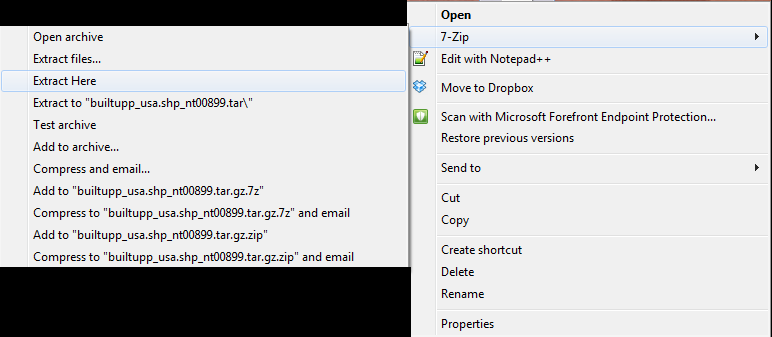
\includegraphics{./Images/7zip_RightClick.png}\\

The resulting file will end in `.tar' Now you need to do one more
de-compression step - right click on the .tar file, select 7-zip, and
`Extract to ``{[}Filename{]}''\,'. This should create a new folder, with
all of the files that were in the compressed folder.

\subsubsection{Dealing with ESRI Geodatabases in QGIS (tested with
version
2.6.1)}\label{dealing-with-esri-geodatabases-in-qgis-tested-with-version-2.6.1}

Some GIS data are only available in a format developed by the company
that makes ArcGIS (ESRI), called ESRI Geodatabases (ESRI .GDB files).
Typically they are used for vector datasets. There are some extra steps
in importing these into QGIS:

\begin{itemize}
\item
  
\includegraphics{./Images/QGIS_AddVectorLayer.PNG}~ Click on the ``Add
  Vector Layer'' icon.
\item
  In the window that pops up, choose the source-type as ``Directory'',
  leave the Encoding set to the default, and change the source to
  ``OpenFileGDB'' (see the example window below).
\item
  Then, click ``Browse'', find and select folder ending in `.gdb', where
  the data are stored (in the example given here, it is the state
  boundary dataset for Arkansas, downloaded from The National Map), and
  click ``Open''.
\end{itemize}

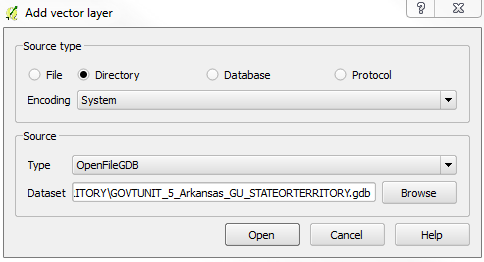
\includegraphics{./Images/QGIS_AddVector_GDB.PNG}\\

\begin{itemize}
\itemsep1pt\parskip0pt\parsep0pt
\item
  Another window will now appear, with a list of layers in this
  geodatabase. You can look at the ``Geometry Type'' to identify whether
  the layer is composed of lines, polygons, or points. If no geometry
  type is identified, the layer may be a table or metadata. You can use
  ``Select All'' to load all layers - this may be a lot of information
  though, so if there are a lot of layers and a large area, you can look
  at one layer at a time.
\end{itemize}

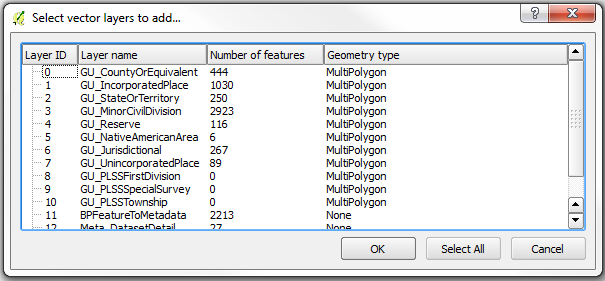
\includegraphics{./Images/QGIS_GDB_Layers.PNG}\\

\begin{itemize}
\itemsep1pt\parskip0pt\parsep0pt
\item
  You cannot edit these layers while they are in .gdb files, but you can
  export them to Shapefiles, and conduct any manipulations/analyses with
  that format.

  \begin{itemize}
  \itemsep1pt\parskip0pt\parsep0pt
  \item
    Right click on the layer you need to work with in the Layers Pane of
    QGIS, and selct ``Save As''.
  \item
    Keep the Format as ESRI Shapefile and define a filename and location
    in the ``Save As'' box. The defaults should work for most purposes.
    The defaults should load the new Shapefile into your current
    project, but you can also use standard data import methods to bring
    the data into QGIS.
  \end{itemize}
\end{itemize}

\subsubsection{Removing Unwanted Features from Vector Layers (e.g.,
isolating a single county of
interest)}\label{removing-unwanted-features-from-vector-layers-e.g.-isolating-a-single-county-of-interest}

Vector datasets may be available for larger areas than you really want -
for example, if you want to work with Tulsa County, Oklahoma, and you
download the appropriate layer from The National Map, the layer you have
will likely include all counties of Oklahoma (and adjacent counties in
neighboring states).

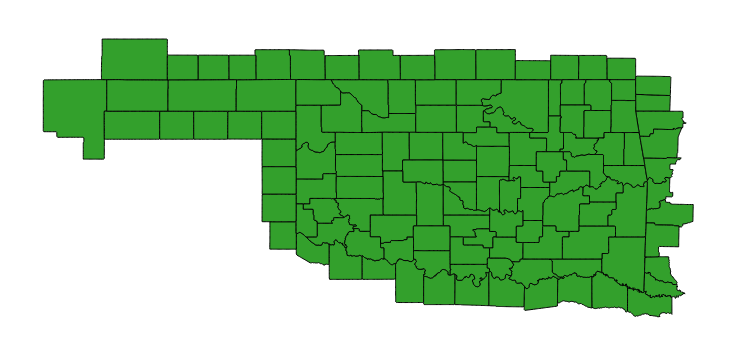
\includegraphics{./Images/OK_Counties.PNG}\\

One way, described below, is to do a query on (i.e., filter out) the
layer to show only the desired features, based on the Attribute Table.
Alternatively, you may make a copy of the shapefile, use the layer
editing tools to delete features. Here are instructions for the former
option, with an example from the ``County or Equivalent'' layer for
Oklahoma, to only display Tulsa County:

\begin{itemize}
\itemsep1pt\parskip0pt\parsep0pt
\item
  Right-click the focal layer and select ``Properties''
\item
  Along the left side of the Properties window, select the ``General''
  tab.
\item
  Make sure the ``Feature subset'' section is open by clicking the arrow
  next to that text, and click the ``Query Builder'' button (see
  screen-shot below).
\end{itemize}

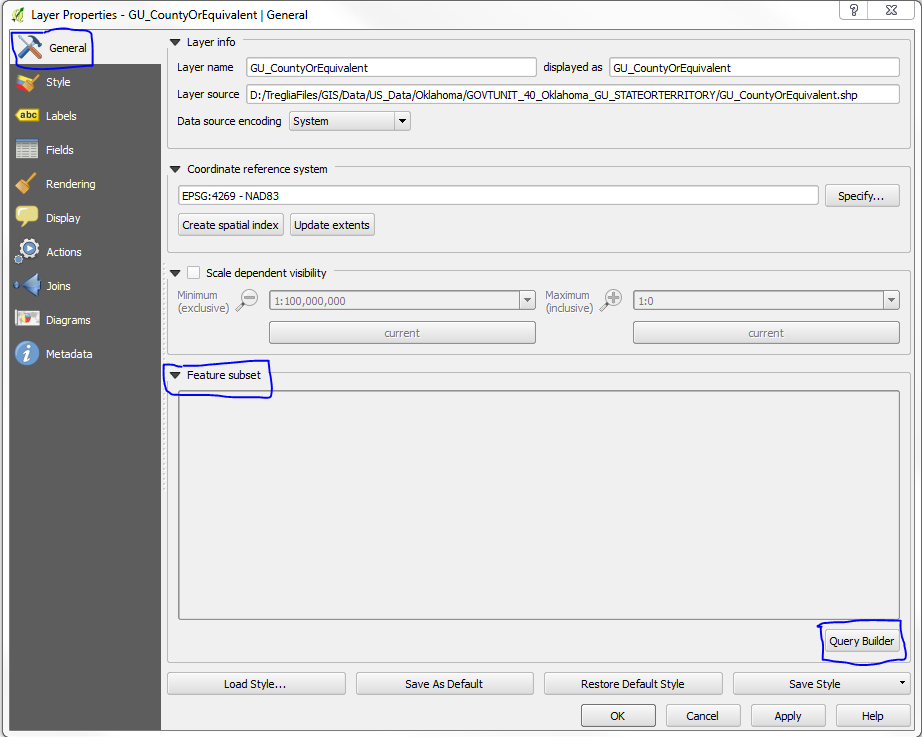
\includegraphics{./Images/QGIS_PropertiesGeneral.PNG}\\

\begin{itemize}
\itemsep1pt\parskip0pt\parsep0pt
\item
  In the next window that appears, there will be an area that says
  ``Fields'' - these are the columns in the Attribute Table for the
  layer. The field ``County\_NAM'' contains the full names of counties.
  An example of the window filled as necessary is provided after this
  section.

  \begin{itemize}
  \itemsep1pt\parskip0pt\parsep0pt
  \item
    If you click a field name, and in the Values box click either
    ``Sample'' or ``All'', either a random sample or all of the possible
    values for the selected attribute will be displayed. So, if you
    select ``COUNTY\_NAM'' and then click ``All'', you will see all of
    the county names listed.
  \end{itemize}
\item
  Double-click the name of the field you wish to filter the data by, and
  it will appear in the white box towards the bottom of this window.
  Then select the appropriate operator you wish to use.

  \begin{itemize}
  \itemsep1pt\parskip0pt\parsep0pt
  \item
    In this case, we wish to select only Counties where the
    ``COUNTY\_NAM'' is ``Tulsa'', so choose the ``='' button. If you
    wanted all counties except for Tulsa, you would use the ``!=''
    button.
  \item
    Then type " `Tulsa' " (or double-click on ``Tulsa'' in list of
    Values).
  \end{itemize}
\item
  If you click ``Test'' with these settings, it should tell you ``The
  where clause returned 1 row(s).'', meaning that only one feature in
  the dataset will be used (i.e., Tulsa County).
\item
  Click ``OK'', then Click ``OK'' again in the Properties window, and
  now Tulsa County is the only area displayed.
\item
  If you need to un-do this, simply get back into the Query Builder
  window, and use the ``Clear'' button towards the bottom.
\end{itemize}

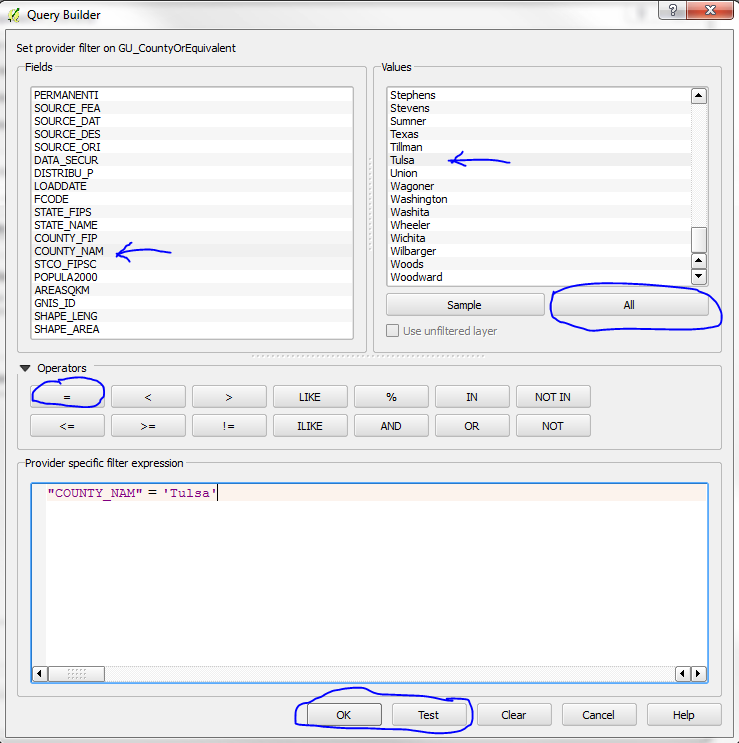
\includegraphics{./Images/QGIS_QueryBuilder.PNG}\\

And here's what the result should look like:


\includegraphics{./Images/OK_TulsaCounty.PNG}\\

\subsubsection{Spatial Reference Information for GIS Data
Layers}\label{spatial-reference-information-for-gis-data-layers}

When you load data into a GIS program, the projection information should
automatically be interpreted by the software, if it is stored correctly
with the relevant files. If the projection information is non-existent,
you may need to look through metadata files that come with the data
(often stored in `.xml' or `.html' documents, labelled as `metadata').
If you find the projection and need to set it in your GIS software, it
may be easiest to do so by filtering for specific terms you find in the
metadata. Furthermore, an internet search for the information you find
in the metadata, with ``EPSG'' code in the search phrase can help you
find a code used in GIS, the EPSG Code. For example, a Google search for
`wgs 84 epsg' returns
\href{http://spatialreference.org/ref/epsg/wgs-84/}{this webpage} as the
first result, and indicates the EPSG code for projected (i.e., global
coordinates of lat/long) in the datum WGS 84 is 4326.

\end{document}
